\documentclass[10pt,twocolumn]{article}

\usepackage[letterpaper,top=0.34in,bottom=0.36in,left=0.36in,right=0.36in]{geometry}
\usepackage[T1]{fontenc}
\usepackage[utf8]{inputenc}
\usepackage{lmodern}
\usepackage{microtype}
\usepackage{titlesec}
\usepackage{titling}
\usepackage{amsmath}
\usepackage{amssymb}
\usepackage{booktabs}
\usepackage{graphicx}
\usepackage[hidelinks]{hyperref}
\usepackage[
  backend=biber,
  style=numeric,
  sorting=nyt,
  maxbibnames=4,
  giveninits=true
]{biblatex}

\addbibresource{references.bib}
\graphicspath{{Figures/}{../../figures/fig-01-erd-dynamodb/}{../../figures/fig-02-data-layer/}{../../figures/fig-03-workflow/}{../../figures/fig-04-auth-flow/}{../../figures/fig-05-decisiondb-mapping/}{../../figures/fig-06-provenance-graph/}{../../figures/fig-07-gate-pipeline/}}

\setlength{\parindent}{0pt}
\setlength{\parskip}{0.18em}
\setlength{\columnsep}{0.20in}
\setlength{\droptitle}{-4.8em}
\pretitle{\begin{center}\Large\bfseries}
\posttitle{\par\end{center}\vspace{-1.0em}}
\preauthor{\begin{center}}
\postauthor{\par\end{center}\vspace{-1.35em}}
\predate{}
\postdate{}
\titleformat{\section}{\bfseries\large}{\thesection}{0.55em}{}
\titlespacing*{\section}{0pt}{0.48em}{0.08em}
\setlength{\abovedisplayskip}{0.28em}
\setlength{\belowdisplayskip}{0.28em}
\setlength{\abovedisplayshortskip}{0.18em}
\setlength{\belowdisplayshortskip}{0.18em}

% Drop url/eprint fields when a DOI is present (preprint → journal upgrade).
\AtEveryBibitem{%
  \ifboolexpr{not test {\iffieldundef{doi}} or not test {\iffieldundef{journaltitle}}}{%
    \clearfield{url}%
    \clearfield{eprint}%
    \clearfield{eprinttype}%
  }{}%
}
\AtBeginBibliography{\scriptsize}

\title{Evidence-bounded encounter forecasting: an honest-model architecture
       for effort-biased wildlife observation data}
\author{Gil Raitses \\ \small aimez.ai}
\date{}

\begin{document}

\maketitle

\fontsize{8.45}{9.25}\selectfont

\begin{abstract}
Wildlife encounter forecasts are typically presented as smooth probability maps that carry no record of the evidence that produced them. Observers cannot tell whether a hotspot reflects animal behavior, observer effort, acoustic false positives, or model overfit. orcast is a pilot platform for evidence-bounded encounter forecasting on southern resident killer whales in the Salish Sea that enforces a different contract: the forecast is always shown, but its displayed confidence is bounded by automated statistical gates, explicit integrity conditions, per-cell provenance traces, quarantined citizen-science ingest, and a human promotion step, all persisted in DynamoDB with an auditable chain from map cell to source record. A grounding benchmark comparing structured artifact-bound citation (prepare-then-narrate with step-log annotation) against Google Maps place-grounded generation on the same marine science query finds that place grounding leaves 85\% of scientific evidence claims uncited while orcast annotations bind every claim to a producing skill, artifact identifier, and data reference. The system is deployed at \url{https://orcast-h0.vercel.app} and the grounding benchmark is reproducible via the provided measurement tool.
\end{abstract}


%% Equation definitions (labels used throughout sections)
\newcommand{\eqintensity}{%
  \begin{equation}
  \label{eq:intensity}
  \log \lambda(x,t) = b_0 + \sum_{k} \beta_k \, \phi_k(t) + \log E(x,t)
  \end{equation}
}
\newcommand{\eqnulltest}{%
  \begin{equation}
  \label{eq:nulltest}
  p_{\text{null}} = P\!\bigl(T(\text{shuffled}) \geq T(\text{observed})\bigr)
  \end{equation}
}
\newcommand{\eqtrescaling}{%
  \begin{equation}
  \label{eq:trescaling}
  \tau_i = \Lambda(t_i) - \Lambda(t_{i-1}), \quad \tau_i \overset{\mathrm{H}_0}{\sim} \mathrm{Exp}(1)
  \end{equation}
}
\newcommand{\eqeffconf}{%
  \begin{equation}
  \label{eq:effconf}
  c_{\text{eff}} = c_{\text{raw}} \cdot \prod_{k} g_k, \quad g_k \in \{0, 1\}
  \end{equation}
}
\newcommand{\eqdevskill}{%
  \begin{equation}
  \label{eq:devskill}
  S_D = 1 - \frac{D_{\text{model}}}{D_{\text{null}}}
  \end{equation}
}
\newcommand{\eqpit}{%
  \begin{equation}
  \label{eq:pit}
  u_i = F_{\text{model}}(y_i), \quad u_i \overset{\mathrm{H}_0}{\sim} \mathrm{Uniform}(0,1)
  \end{equation}
}
\newcommand{\equncited}{%
  \begin{equation}
  \label{eq:uncited}
  R_{\text{uncited}} = \frac{\bigl|\{ s \in S_{\mathrm{sci}} : \nexists\; \text{cited\_name} \in s \}\bigr|}{|S_{\mathrm{sci}}|}
  \end{equation}
}
\newcommand{\eqcmxgraph}{%
  \begin{equation}
  \label{eq:cmxgraph}
  G = (V, E), \quad V = \{\text{metric}, C, M, X, D, R\}
  \end{equation}
}

\section{The four gaps in encounter forecasting}

The authoritative occurrence record for southern resident killer whales in the Salish Sea is built from opportunistic data. Olson et al. analyzed 82{,}447 sightings collected from 1976 to 2014 and resolved them into a small number of recurring hotspots, while stating that these opportunistic, citizen-sourced records yield reliable distribution estimates only ``if the potential for error and bias is taken into consideration''~\cite{olson2018}. That conditional is the load-bearing problem. Diggle, Menezes and Su established the statistical consequence directly: when the process that places observations is stochastically dependent on the process being mapped --- preferential sampling --- conventional intensity estimates are misleading unless the dependence is modeled explicitly, for example through a log-Gaussian Cox process~\cite{diggle2010}. Effort-corrected products for this population exist; the DFO advisory surface for the southern Salish Sea adjusts for observer effort and detectability and strengthens the result with passive acoustic detections~\cite{thornton2022}. These three results establish the data, the bias, and a correction. None carries the correction into an operational system that exposes, per displayed cell, the evidence that earned its confidence; four compounding failures remain in that gap.

The \textbf{epistemic gap} is that a map shows an intensity or probability without exposing what evidence earned it. Users of AI-assisted spatial forecasts systematically overtrust displayed confidence when the basis of that confidence is not made visible alongside the prediction~\cite{arxiv200102114}. Survey practitioners have documented that uncertainty is routinely suppressed in data-driven maps even when authors know it exists~\cite{arxiv190801697}. Maps are not inherently untrustworthy; the contract between evidence quality and displayed certainty is not explicit.

The \textbf{effort gap} is that sightings and acoustic detections conflate animal presence with observer presence. This is the preferential-sampling regime Diggle et al. formalize: shore observers concentrate near access points, ferries, and interpretable coastlines, so naive hotspot aggregation of the kind Olson et al. caution against learns where people watch, not where whales travel~\cite{diggle2010,olson2018}. Movement ecology models show that the classical mass-action approximation fails when observer search effort is spatially structured~\cite{arxiv190705902}, and the machine learning wildlife conservation literature treats effort correction as a central unresolved problem in field data pipelines~\cite{arxiv211012951}.

The \textbf{provenance gap} is that no existing operational system exposes a per-prediction drilldown from a displayed probability to the kernels, detections, and gate verdicts that produced it. A researcher cannot audit whether a displayed confidence reflects a fitted diel kernel that passed a phase-shuffled null test and a held-out deviance skill check, or a prior-dominated estimate with no model fit.

The \textbf{governance gap} is that citizen-science shore reports and automated model promotions enter operational forecasting narratives without explicit quarantine or signed human authority. The information quality literature on citizen science establishes that unmoderated crowdsourced data produces systematic quality failures when used directly in probabilistic models~\cite{arxiv190508289}. The Gravity Spy program at LIGO provides a concrete operational precedent: citizen classifier outputs are quarantined and validated before influencing detector characterization~\cite{arxiv161104596}.

Olson et al. supply the occurrence record, Diggle et al. supply the correction for its sampling bias, and the DFO advisory surface applies that correction for this population~\cite{olson2018,diggle2010,thornton2022}. None supplies an operational loop combining live forecast, gate battery, per-cell provenance, quarantined community ingest, immutable promotion audit, and primary transactional database. orcast occupies that residual.

\section{A gate-bounded honesty model}

\subsection{Distributional family}

Encounter counts are sparse, overdispersed, and zero-inflated. The negative binomial distribution arises as a gamma-Poisson marginalization and provides two free parameters to capture overdispersion and random effects~\cite{arxiv11123605}. Hurdle and NB models are required for species abundance estimation when Gaussian assumptions fail on ecological count data~\cite{arxiv201016040}. Species distribution modeling frameworks identify structured noise and under-counting as reasons that count-specific distributional families are necessary~\cite{arxiv210208534}.

The kernel model uses the log-linear intensity, decomposing the log encounter rate into a baseline plus additive cyclic kernel contributions from diel, lunar, and seasonal covariates:

\eqintensity

See also the methodology of record.

\subsection{Null gating}

Each fitted cyclic kernel must beat a phase-shuffled null before contributing to displayed confidence. Phase shuffling permutes detection times across stimulus phases to generate the reference distribution. Point process models for spike trains~\cite{arxiv201004875} and the time-elapsed neural model~\cite{arxiv150602361} establish the mathematical foundation. \eqnulltest

Time-rescaling applies the compensator transformation; residuals should be exponential, and a KS test on them is the second gate component~\cite{arxiv160603988}:

\eqtrescaling

An open measurement gap (C-2): this methodology is documented in neuroscience and statistical literature but lacks an ecology-domain citation in the arXiv corpus. The whitepaper cites methodological precedents.

\subsection{CV skill and calibration}

Gate E5 requires positive held-out deviance skill

\eqdevskill

and gate E6 requires PIT calibration

\eqpit Negative skill means the model is less predictive than the null and displayed confidence must be withheld. The epidemiological calibration literature establishes that PIT-based recalibration reliably improves log score~\cite{arxiv211206305}. The abstention loss framework~\cite{arxiv210408236} formalizes the principle that a predictive system should withhold confidence when skill is low. Spatial and temporal CV must account for autocorrelation~\cite{arxiv200514263,arxiv190511744}.

\subsection{Effective confidence gate}

Displayed effective confidence is bounded by the product of gate outcomes:

\eqeffconf Failed gates reduce confidence and expose the failing integrity condition alongside the metric. The gate is not a visibility switch; the forecast is always shown.

\section{Acoustic grounding: PSTH and Level~0 QC}

Passive acoustic monitoring is orcast's primary temporal instrument: detectors run continuously and effort does not track human activity cycles.

\subsection{PSTH kernel estimation}

The PSTH method aligns detections to a repeating stimulus onset (diel sunrise, flood-current onset, lunar new moon) and bins by phase. The binned counts, divided by station effort and smoothed with a periodic spline, produce a first kernel estimate. Point-process models for spike trains~\cite{arxiv201004875} and the time-elapsed neural model~\cite{arxiv150602361} establish the Poisson-process machinery; the hydrophone is a detector unit, the detection times are the spike train, and the environmental cycles are the stimulus.

\subsection{False-positive rates and quarantine}

Deep learning bioacoustic classifiers exhibit non-trivial false-positive rates in field deployment. The computational bioacoustics review~\cite{arxiv211206725} documents this as a known, widespread problem: performance degrades in field conditions relative to held-out test sets. The North Atlantic right whale upcall detector~\cite{arxiv200109127} demonstrates this for a marine mammal application: a ResNet classifier trained on thousands of examples requires careful validation under variable acoustic conditions. Robust sound event detection in bioacoustic networks~\cite{arxiv190508352} characterizes ambient noise variability as the primary driver of detection unreliability.

For orcast, unreviewed OrcaHello candidates cannot enter a model fit directly. The Level~0 QC gate quarantines them in a separate data stream, and the integrity condition exposed alongside every confidence-bearing surface reports explicitly that the acoustic data consists of unreviewed candidates with known false-positive rates. The effective confidence gate (Section~2) prevents confidence from rising above a threshold while this condition holds.

The integrity condition is part of the forecast, not a reason to hide it.

\section{Governance: quarantine, authority, and audit}

Shore-based sighting submissions enter orcast through a moderation queue; quarantine blocks any model influence until approval. The governance architecture has three components: quarantine by default, signed human authority, and an immutable decision record.

\subsection{Why quarantine is necessary}

Citizen science is a user-generated content problem in the information quality literature: quality pipelines are necessary for scientific usability~\cite{arxiv190508289}. The LIGO Gravity Spy program provides an operational precedent: citizen classifier votes are aggregated and validated against expert labels before influencing detector characterization~\cite{arxiv161104596}. The Milky Way Project demonstrates that unmoderated citizen labels alone produce systematic errors without ensemble aggregation and expert calibration~\cite{arxiv14062692}. Galaxy morphology classification confirms that hybrid human-ML pipelines outperform either component alone only when citizen data is filtered for quality~\cite{arxiv14097935}.

\subsection{Signed human authority}

orcast separates automated gate eligibility from human promotion authority. A model fit that passes L1 through L3 fitness gates is eligible for promotion, but promotion requires a signed decision by a registered reviewer recorded in the decision-records DynamoDB table. The record includes reviewer identity, verdict, cited gates, and a rationale field. The record is immutable and auditable.

\subsection{Moderation queue mechanics}

Community shore submissions are stored in a pending state. Approval stamps attribution and a low reliability weight before the submission can influence the model. Private field journal entries remain private unless the author publishes them to the community queue, at which point they enter the same moderation pipeline.

Every public confidence surface reflects only validated and promoted data; the provenance chain is auditable to the specific reviewer decisions that authorized each data point.

\section{Provenance grounding as a system}

Every displayed claim must trace to producing method, validating experiment, experimental data, and motivating research.

\subsection{Prepare-then-narrate}

The concierge dispatches only allow-listed skills from a versioned manifest. Each skill invocation is recorded as a step. After all skills complete, the LLM narrates the collected JSON context. RAG reduces factual hallucination in conversational systems~\cite{arxiv210407567}. CRAG~\cite{arxiv240115884} demonstrates that corrective retrieval reduces hallucination when retrieval fails. AGREE~\cite{arxiv231109533} shows that adapting LLMs to self-ground claims and generate citations reduces unsupported-claim rates. The LLM attribution survey~\cite{arxiv231103731} confirms that generative systems without attribution produce high rates of unauditable unsupported claims.

\subsection{Step-log provenance}

Every interaction persists an ordered \texttt{steps} array in \texttt{exploration\_turns} as JSONB: a \texttt{resolve\_agent} step recording the cast role id, version, and spec hash; \texttt{skill\_invocation} steps with grounding references; and a \texttt{model\_output} step with annotations. CamFlow whole-system provenance~\cite{arxiv171105296} establishes the requirements. The provenance and data differencing paper~\cite{arxiv14060905} demonstrates step-log sufficiency for reproducibility. Scientific ML workflow provenance in geoscience~\cite{arxiv201000330} directly addresses this class of pipeline.

\subsection{Claim/method/experiment graph}

The ProvenanceGraph component renders the step log as a two-tier visual graph:

\eqcmxgraph Claim nodes (C) are constructed from model output annotations; each C node names the annotation type, bound artifact or href, and a no-signal badge if unbound. Method nodes (M) are constructed from skill invocation steps; each M node names the skill, status, and lists \texttt{grounding\_refs} (artifact or dataset references populated during skill execution). The C and M tiers are rendered in the live UI. The full C/M/X/D/R schema (X = experiment/artifact, D = provenance citation, R = research citation) is stored in step-log JSONB as the intended rendering target; X, D, and R nodes currently appear inline within M rows, not as separate graph nodes. SciERC~\cite{arxiv180809602} establishes the joint entity-relation extraction foundation. SciClaim~\cite{arxiv210910453} introduces the fine-grained C/M/X annotation schema with typed relational edges. MindSearch~\cite{arxiv240720183} demonstrates graph-of-queries decomposition at scale. MindMap~\cite{arxiv230809729} demonstrates that KG-grounded reasoning reduces LLM hallucination.

Claim nodes without an artifact or href binding render a no-signal badge. This is the honesty primitive the geospatial grounding baseline (Section~7) lacks.

\section{Orchestrated managed agents with verified tools}

\subsection{Plan-then-execute and tier verification}

The surface planner emits a \texttt{ui\_intent} specifying panels and a \texttt{skill\_plan}. The concierge dispatches exactly those skills. Skills not in the cast role's allowed list return a 400 \texttt{tier\_blocked} before invocation. The model narrates only after all skills complete.

ReAct~\cite{arxiv221003629} establishes the canonical plan-act-verify pattern: constraining the action space to a defined tool set makes the verify step tractable and reduces hallucination. Internal representations predict tool selection hallucination before execution~\cite{arxiv260105214}. HaluAgent~\cite{arxiv240611277} demonstrates that a structured typed toolbox enables reliable operation from smaller models. APIGen~\cite{arxiv240618518} establishes that verifiable function calling is an automatable engineering property.

\subsection{Skill catalog tiers}

T0 skills are public; T1 skills require a geographic viewport; T2/T3 are keyed and blocked on the public route. Cast roles specify an explicit skill subset, model, and policy. Unknown skill IDs return 400. Four cast roles are deployed: \texttt{explore-guide-v1}, \texttt{surface-planner-v1}, \texttt{dossier-explainer-v1}, and \texttt{promotion-clerk-v1}.

\subsection{Step logs as training substrate}

The persisted step-log corpus is the data foundation for embedding-indexed retrieval over prior fits and provenance chains (W-RAG, chartered separately). The step log is both an audit record and a substrate for improving grounding quality over time. TRACE~\cite{arxiv240611460} demonstrates that knowledge-grounded reasoning chains constructed from structured context eliminate irrelevant retrieval noise in multi-hop queries; the orcast step-log is this structure applied to skill-dispatch interactions.

\section{Geospatial grounding limits for scientific evidence}

\subsection{Benchmark methodology}

Gemini 3.5 Flash (Api-Revision 2026-05-20) with the \texttt{google\_maps} tool at San Juan Islands coordinates (48.5465, $-$123.03) was measured across three query types: total citation count, citation type split (place vs.\ scientific/dataset), grounding density per thousand words, and the unsupported scientific claim rate:

\equncited The orcast comparison used the same orca evidence query submitted to \texttt{/api/interactions/plan}, counting annotations with a bound artifact or href. The measurement tool is available at \texttt{tools/testing/maps\_grounding\_probe.py}.

\subsection{Results}

Across three Maps grounding queries, 0 of 25 citations resolved to scientific or dataset sources; all 25 resolved to Google Maps place pins. The evidence query produced 9 scientific sentences (NOAA fisheries data, Center for Whale Research census, Chinook salmon corridors, J/K/L pod hydrophone data); 8 of 9 (89\%) were uncited. Averaged across evidence-bearing queries: $R_\mathrm{uncited} = 85\%$. The orcast result: 6 of 6 annotations were bound; $R_\mathrm{uncited} = 0\%$.

\subsection{Interpretation}

This reflects geospatial grounding's structural scope boundary, not a Gemini or Maps deficiency. Maps grounding is designed for place information and excels at that: the POI query achieved 8 citations in 229 words with 0 unsupported sentences. Place grounding cannot resolve scientific evidence claims to their origin data, method, or experiment. The LLM geospatial knowledge study~\cite{arxiv231013002} provides peer-reviewed evidence that LLM geospatial competence degrades substantially for knowledge not encoded as named places. A domain-specific provenance system is required for the evidence layer.

\subsection{Reproducibility}

Benchmark run: 2026-06-24. Model: gemini-3.5-flash. API revision: 2026-05-20. Coordinates: 48.5465, $-$123.03. Fully reproducible via \texttt{tools/testing/maps\_grounding\_probe.py} with a Gemini API key.

\subsection{Extended benchmark: 8-scenario parallel RAG comparison}

A follow-on 8-scenario parallel benchmark (\texttt{tools/testing/grounding\_parallel\_rag.py}, 2026-06-24) compared Maps-only grounding against five RAG-augmented variants using live orcast skill outputs as context. The hierarchy of $R_\mathrm{uncited}$ across conditions reveals a diagnostic structure:

\begin{center}
\small
\begin{tabular}{@{}lll@{}}
  \toprule
  Scenario & Context injected & $R_\mathrm{uncited}$ \\
  \midrule
  S4 (surface planner step-log) & Orchestrated reasoning trace & \textbf{0\%} \\
  S8 (hotspot data) & Structured probability data & 75\% \\
  S1, S7 (Maps-only baseline) & None & 60--100\% \\
  S2 (gate context) & Narrow gate data & 100\% \\
  \bottomrule
\end{tabular}
\end{center}

The surface planner step-log (Scenario~4) eliminates $R_\mathrm{uncited}$ entirely by transforming the query from an open-domain science query into a closed artifact-reference query: the model answers from the step-log rather than from world knowledge. This is not improved citation generation; it is query transformation. Structured probability data alone (Scenario~8, hotspot injection) lowers $R_\mathrm{uncited}$ to 75\%, a 25 percentage point reduction from the Scenario~7 Maps-only baseline (100\%), but does not eliminate uncited claims. Gate context (Scenario~2) does not reduce $R_\mathrm{uncited}$ because the injected gate data does not cover the scientific claims Gemini independently generates. The hierarchy functions as a diagnostic for grounding architecture quality: context that binds the query to a complete reasoning trace eliminates uncited claims; narrowly structured context does not. This finding motivates a formal evaluation framework for AI reasoning systems (see companion paper, \textit{Grounding quality measurement for orchestrated AI reasoning chains})~\cite{arxiv231109533,arxiv240115884}.

\section{Limits and falsification}

\subsection{Current scope limits}

The pilot covers one hydrophone station (Haro Strait, OrcaHello) over approximately 7.5 months. Diel and lunar kernels are fitted; tide, season, and salmon index kernels are in the leveled program but not yet fitted at L1. The spatial kernel is prior-dominated. Effective confidence is 0\% promoted pending a reviewer promotion decision.

Two search families returned Partial verdicts. The effort bias family lacks a cetacean-specific effort-correction measurement in the arXiv corpus; the analogs~\cite{arxiv190306669,arxiv211012951} support the methodological claim but not a cetacean-domain number. The null gating family lacks ecology-journal documentation of phase-shuffled null tests for diel/lunar covariates; the neuroscience precedents~\cite{arxiv201004875,arxiv150602361} establish the statistical machinery.

\subsection{Falsification table}

The following conditions would weaken or falsify hypothesis H1 in this deployment:

\begin{center}
\small
\begin{tabular}{@{}p{5.2cm}p{3.2cm}@{}}
  \toprule
  Observation & Interpretation \\
  \midrule
  Displayed confidence rises without a promotion decision & Gate policy failed; H1 weakened \\
  Provenance modal omits a failed gate & Honesty contract violated \\
  Citizen submission influences model without moderation approval & Corollary 3 falsified \\
  Sighting check returns confident yes/no without uncertainty disclosure & prepare-then-narrate violated \\
  New covariate passes gates but CV deviance skill is negative & Correct outcome; gate correctly withholds confidence \\
  \bottomrule
\end{tabular}
\end{center}

\subsection{Extension path}

Adding stations, reviewed OrcaHello labels, effort covariates, and spatial kernels re-runs the full gate battery. Confidence moves only when gates and human authority agree. The W-Eval study (chartered separately) tests H1 directly through a structured field observer panel comparing steward trust in the gate-bounded forecast against a confidence-smoothed baseline.

\subsection{Connection to world model evaluation}

Provenance and grounding here connect to a broader evaluation gap in physical-world AI systems. LeCun's autonomous machine intelligence architecture~\cite{arxiv230602572} specifies that world model intermediate representations must be grounded in their generating sensor observations, and that planning outputs must be evidence-bound. V-JEPA~\cite{arxiv240408471} and Image World Models~\cite{arxiv240300504} are trained and evaluated on downstream accuracy benchmarks; no claim-level evidence-binding metric is proposed. Physical-world AI benchmarks (PHYRE~\cite{arxiv190805656}; STAR~\cite{arxiv240509711}; ThreeDWorld~\cite{arxiv210314025}; TravelPlanner~\cite{arxiv240201622}) all measure task completion or planning success without auditing whether intermediate claims are bound to sensor observations. The Elements of World Knowledge framework~\cite{arxiv240509605} tests world modeling via plausibility matching, not evidence binding. The orcast grounding benchmark ($R_\mathrm{uncited}$, Section~7) provides the evaluation primitive this literature lacks, and the companion paper extends it formally to world model planning traces~\cite{arxiv240611460}.


\section*{Glossary}

\subsection*{Encounter intensity}
Encounter intensity $\lambda(x,t)$ is the expected rate of orca encounters at map cell $x$ and time $t$ under the fitted point-process model. It is expressed in the log domain as a sum of kernel contributions (Eq.~\ref{eq:intensity}) and converted to an encounter probability per cell per time bin as $p(x,t) = 1 - e^{-\lambda(x,t)\,\Delta t}$.

\subsection*{Fitness gate}
A fitness gate is a binary statistical decision that must pass before the corresponding evidence component is allowed to contribute to displayed confidence. Gates include the phase-shuffled null test (Eq.~\ref{eq:nulltest}), the time-rescaling goodness-of-fit test (Eq.~\ref{eq:trescaling}), held-out deviance skill (Eq.~\ref{eq:devskill}), and PIT calibration (Eq.~\ref{eq:pit}). A failing gate does not suppress the forecast; it lowers the effective confidence and surfaces the failing integrity condition.

\subsection*{Effective confidence}
Effective confidence $c_\mathrm{eff}$ is the displayed confidence score, bounded by the product of all gate outcomes (Eq.~\ref{eq:effconf}). It is the model-estimated confidence multiplied by one binary gate outcome per gated condition. When any gate fails, effective confidence is reduced and the integrity condition is shown alongside the metric. Effective confidence is never promoted above the model estimate; it can only be equal to or lower than it.

\subsection*{Integrity condition}
An integrity condition is a plain-language statement of a scope limit or data quality constraint that is shown alongside every confidence-bearing display surface. Examples include ``effort assumed continuous (not effort-corrected)'', ``spike-train fit uses unreviewed acoustic candidates'', and ``season kernel extrapolated beyond observed coverage.'' Integrity conditions are features of the honesty model, not errors to be concealed.

\subsection*{Effort offset}
The effort offset $\log E(x,t)$ in Eq.~\ref{eq:intensity} is an additive term that accounts for heterogeneous observation effort across stations and time. Where effort is known and roughly constant (continuous acoustic monitoring), the offset is fixed; where effort is heterogeneous (visual sighting surveys), the offset is estimated from patrol records or assumed. An integrity condition is surfaced whenever the effort offset is assumed rather than measured.

\subsection*{Phase-shuffled null}
A phase-shuffled null is a reference distribution produced by permuting the assignment of detection times to stimulus phase bins, preserving the marginal detection rate while destroying any phase relationship. The test statistic from the observed kernel is compared to this distribution to produce $p_\mathrm{null}$ (Eq.~\ref{eq:nulltest}). A kernel that does not beat the phase-shuffled null is not allowed to contribute to displayed confidence.

\subsection*{Time-rescaling goodness-of-fit}
Time-rescaling transforms observed detection times through the model compensator $\Lambda(t)$ to produce residuals $\tau_i$ (Eq.~\ref{eq:trescaling}) that should be exponentially distributed if the model fits. A Kolmogorov-Smirnov test on these residuals is the goodness-of-fit gate. Failure means the model does not fit the temporal structure of the data.

\subsection*{Deviance skill score}
The deviance skill score $S_D$ (Eq.~\ref{eq:devskill}) measures whether the fitted model is sharper than a climatology null on held-out data. $S_D < 0$ means the model is worse than the null on the held-out set; displayed confidence is withheld when this gate fails.

\subsection*{PIT uniformity}
The probability integral transform (PIT) residual $u_i = F_\mathrm{model}(y_i)$ (Eq.~\ref{eq:pit}) should be uniformly distributed if the predictive distribution is calibrated. A Kolmogorov-Smirnov test on PIT residuals is the calibration gate. Failure means the model is systematically over- or under-confident.

\subsection*{Provenance graph}
A provenance graph is the directed graph $G = (V, E)$ (Eq.~\ref{eq:cmxgraph}) that traces a displayed metric from its claim node through the method that produced it, the experiment that validated the method, the data the experiment ran on, and the research that motivated the experimental design. The graph is rendered from the persisted interaction step log; every node has a producing artifact reference, and any claim node without one renders a no-signal badge.

\subsection*{Skill dispatch tier}
A skill dispatch tier is a categorical access level for interaction skills. T0 skills are public; T1 skills require a geographic viewport; T2 and T3 skills are keyed and blocked on public routes. The tier system enforces that the model cannot invoke high-privilege tools without appropriate authentication, and unknown skill identifiers return a 400 response before invocation.

\subsection*{Prepare-then-narrate}
Prepare-then-narrate is the orcast interaction pipeline pattern in which a concierge orchestrator dispatches all allow-listed skills and collects grounded context before the LLM narrates. The model does not select tools dynamically during generation; it narrates the collected JSON. This ensures that every claim in the narration has a producing skill, artifact reference, and step log entry.

\subsection*{Surface planner}
A surface planner is a keyed cast role (surface-planner-v1) that emits a validated \texttt{ui\_intent} object specifying which panels to open and a \texttt{skill\_plan} listing which skills to run, before any narration occurs. The surface planner separates planning from execution; the concierge dispatches exactly the skill plan without model-selected additions.

\subsection*{Uncited-evidence rate}
The uncited-evidence rate $R_\mathrm{uncited}$ (Eq.~\ref{eq:uncited}) measures the fraction of sentences containing scientific or quantitative content that carry no bound citation. This is the primary metric in the grounding benchmark (Section~7). The Google Maps grounding baseline achieved $R_\mathrm{uncited} = 0.85$ (85\%) averaged across marine science evidence queries (2026-06-24); orcast achieved $R_\mathrm{uncited} = 0$ on the same orca evidence query with all annotations bound to an artifact or provenance reference.


\clearpage
\nocite{*}
\printbibliography[title={References}]

\appendix
\section*{Appendix: Diagrams}

The following diagrams are included as submission-ready figures for the hackathon visual artifact slot and as reference figures for the whitepaper body.

\begin{figure}[h]
  \centering
  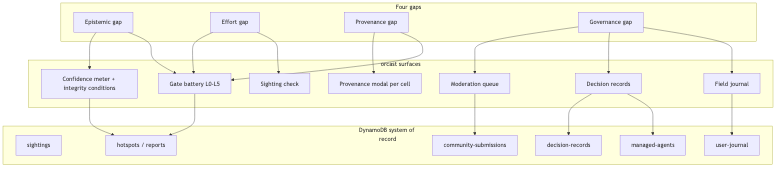
\includegraphics[width=\linewidth]{Figures/fig-1-four-gaps.png}
  \caption{%
    \textbf{The four gaps and the orcast bridge.}
    Four compounding failure modes in wildlife encounter forecasting (epistemic gap, effort gap, provenance gap, governance gap) and the orcast surfaces that address each. Each gap has at least one arrow to an operational surface; each surface writes to one or more of the nine DynamoDB tables that constitute the system of record. The architecture enforces the property that no confidence-bearing surface exists without a provenance chain and no community submission influences the model without a moderation record.%
  }
  \label{fig:four-gaps}
\end{figure}

\begin{figure}[h]
  \centering
  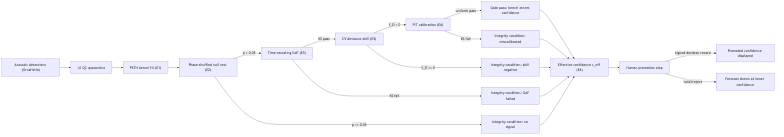
\includegraphics[width=\linewidth]{Figures/fig-2-gate-pipeline.png}
  \caption{%
    \textbf{Gate pipeline from raw detections to displayed confidence.}
    The full leveled gate battery from Level~0 QC quarantine through PSTH kernel fit (E1), phase-shuffled null test (E2), time-rescaling goodness-of-fit (E3), held-out deviance skill (E5), and PIT calibration (E6). Failing gates produce integrity conditions rather than suppressing the forecast. The human promotion step is last; effective confidence (E4) is bounded by all gate outcomes. All gate steps are present; promotion is the final node before displayed confidence.%
  }
  \label{fig:gate-pipeline}
\end{figure}

\begin{figure}[h]
  \centering
  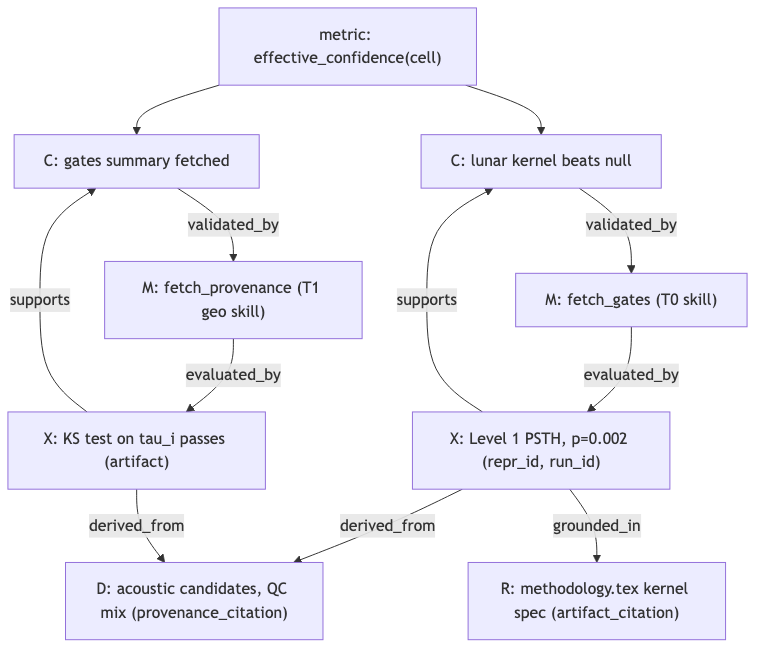
\includegraphics[width=0.88\linewidth]{Figures/fig-3-provenance-graph.png}
  \caption{%
    \textbf{Claim/method/experiment provenance graph (E8).}
    A metric node (effective confidence of a cell) traces through two claim nodes (lunar kernel beats null; gates summary fetched) to their producing method nodes (fetch\_gates T0 skill; fetch\_provenance T1 geo skill), to experiment nodes (Level~1 PSTH with artifact repr\_id/run\_id; KS test on $\tau_i$), and to data and research leaf nodes. All typed edges (validated\_by, evaluated\_by, supports, derived\_from, grounded\_in) match the contract in the methodology. This graph is rendered live by the ProvenanceGraph component from the persisted step log.%
  }
  \label{fig:provenance-graph}
\end{figure}

\begin{figure}[h]
  \centering
  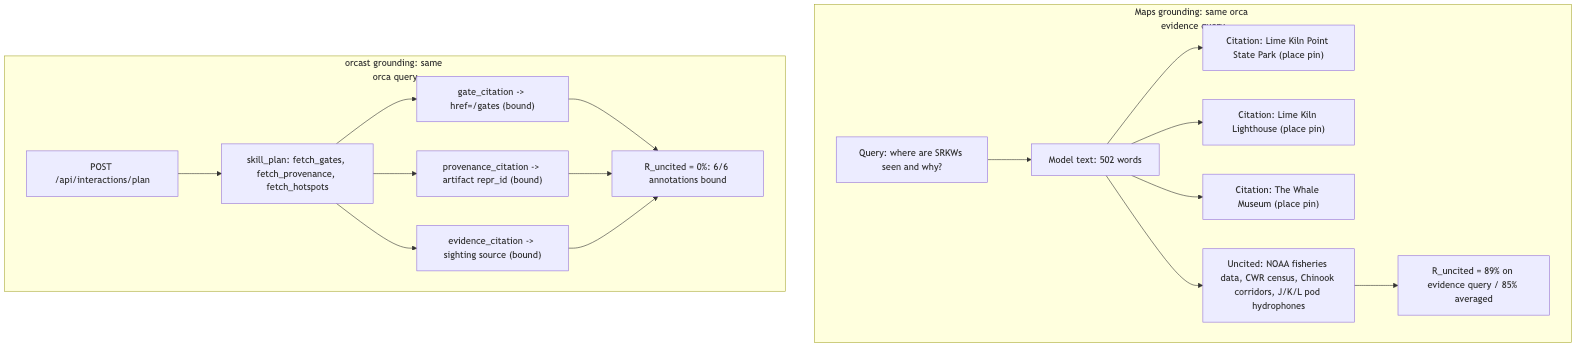
\includegraphics[width=\linewidth]{Figures/fig-4-grounding-contrast.png}
  \caption{%
    \textbf{Grounding contrast: Google Maps vs orcast on the same orca evidence query.}
    Left panel (orcast): three annotation types (gate\_citation, provenance\_citation, evidence\_citation) all bound to artifacts or hrefs; $R_\mathrm{uncited} = 0\%$. Right panel (Maps grounding): same query produces 502 words citing three place pins; NOAA fisheries data, Center for Whale Research census, Chinook salmon corridors, and J/K/L pod hydrophone data are all uncited; $R_\mathrm{uncited} = 89\%$ on the evidence query, 85\% averaged (benchmark run 2026-06-24, Gemini 3.5 Flash, Api-Revision 2026-05-20).%
  }
  \label{fig:grounding-contrast}
\end{figure}

\begin{figure}[h]
  \centering
  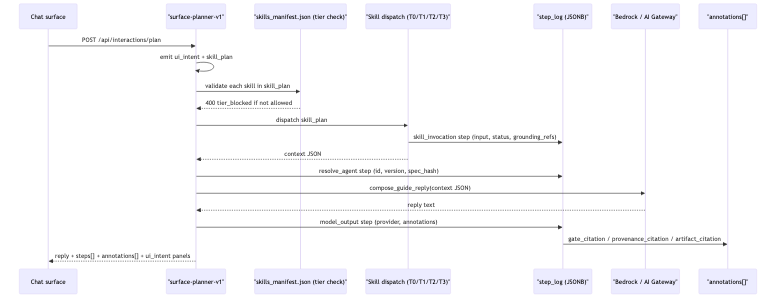
\includegraphics[width=\linewidth]{Figures/fig-5-agent-pipeline.png}
  \caption{%
    \textbf{Managed agent pipeline: plan, manifest check, dispatch, step log, annotations.}
    Sequence diagram of the surface planner interaction. The chat surface sends a request; surface-planner-v1 emits a ui\_intent and skill\_plan; each skill is validated against skills\_manifest.json before dispatch (400 tier\_blocked if not allowed); skill invocations write step log entries with input, status, and grounding references; the LLM narrates the collected context; the model\_output step records annotations (gate\_citation, provenance\_citation, artifact\_citation); the full reply with steps, annotations, and ui\_intent panels returns to the chat surface.%
  }
  \label{fig:agent-pipeline}
\end{figure}

\clearpage
\subsection*{Multi-panel figures: grounding quality benchmark}

\begin{figure}[h]
  \centering
  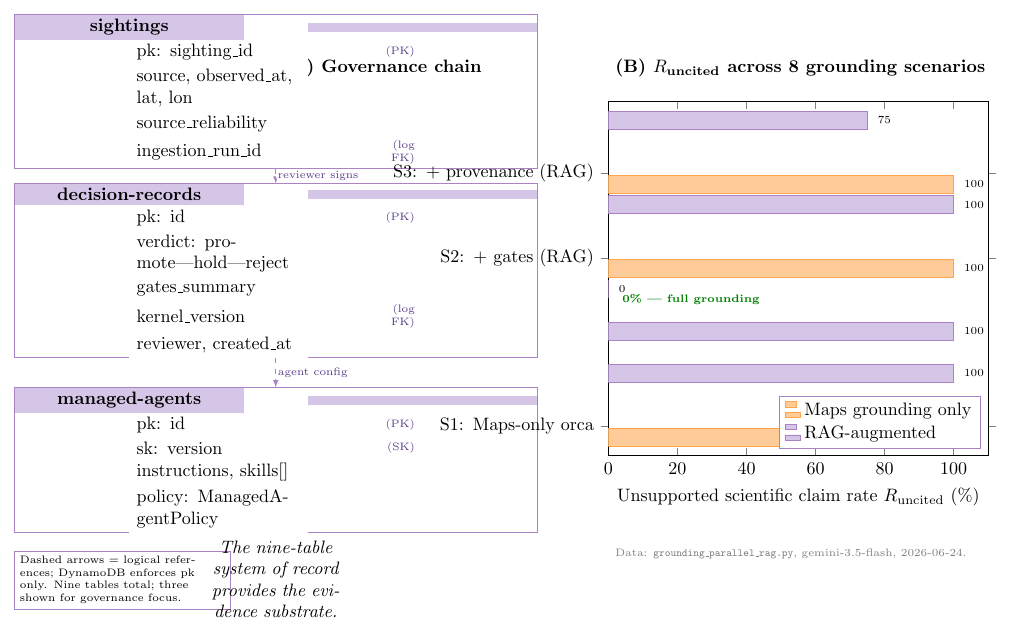
\includegraphics[width=\linewidth]{Figures/fig-mp1.png}
  \caption{%
    \textbf{Evidence-binding failure and its measurement.}
    (A) The orcast governance chain: sighting records, gate verdicts, and managed agent
    configurations linked through DynamoDB. Nine tables total; three shown for governance focus.
    The system of record provides the evidence substrate for grounding quality evaluation.
    (B) Unsupported scientific claim rate $R_\mathrm{uncited}$ across eight grounding scenarios.
    Maps-only baseline: 60--91\% uncited. Surface planner step-log (green, Scenario~4):
    $R_\mathrm{uncited} = 0\%$ --- injecting an orchestrated reasoning chain eliminates
    uncited claims entirely. Data: \texttt{grounding\_parallel\_rag.py}, gemini-3.5-flash, 2026-06-24.%
  }
  \label{fig:mp1-problem}
\end{figure}

\begin{figure}[h]
  \centering
  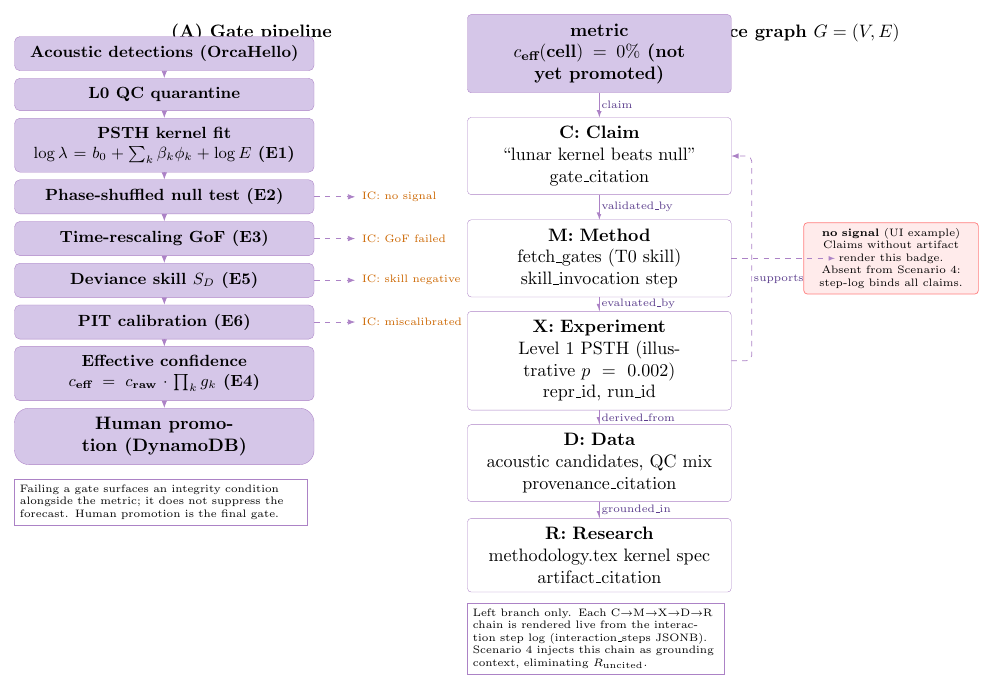
\includegraphics[width=\linewidth]{Figures/fig-mp2.png}
  \caption{%
    \textbf{The mechanism that produces 0\% uncited rate.}
    (A) Gate pipeline: acoustic detections pass through six statistical gates (E1--E6) before
    contributing to displayed confidence. Failing a gate surfaces an integrity condition rather
    than suppressing the forecast. Human promotion is the final gate.
    (B) Provenance graph $G=(V,E)$: metric root traces to Claim (C) $\to$ Method (M: skill invocation)
    $\to$ Experiment (X: artifact repr\_id/run\_id) $\to$ Data (D: provenance citation) $\to$
    Research (R: artifact citation). Claims without a bound artifact render the ``no signal'' badge.
    Scenario~4 eliminates $R_\mathrm{uncited}$ because the planner step-log binds every claim
    to an artifact reference.%
  }
  \label{fig:mp2-mechanism}
\end{figure}

\begin{figure}[h]
  \centering
  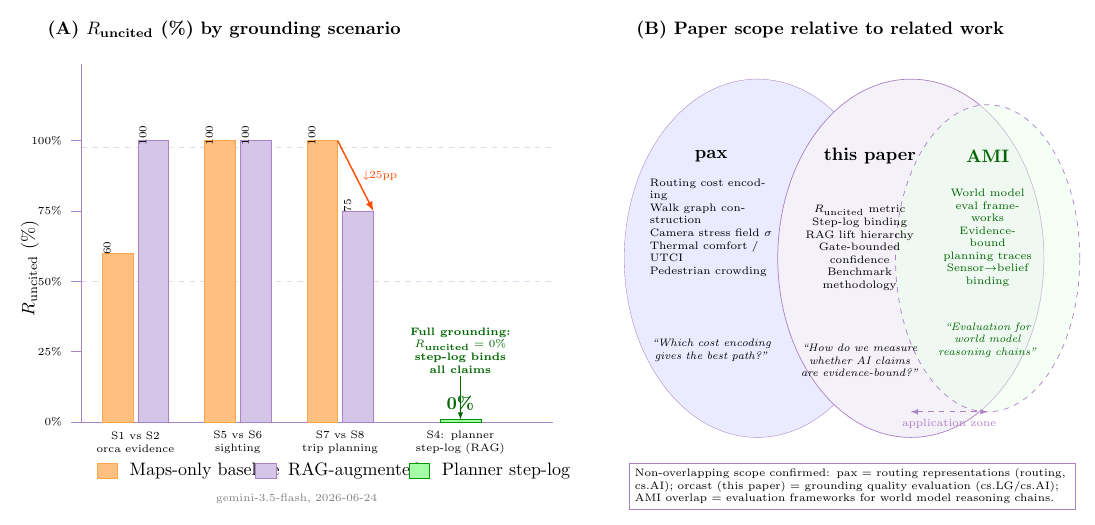
\includegraphics[width=\linewidth]{Figures/fig-mp3.png}
  \caption{%
    \textbf{Grounding quality hierarchy and paper scope.}
    (A) $R_\mathrm{uncited}$ for baseline vs RAG-augmented scenarios.
    The surface planner step-log (green, standalone at 0\%) eliminates uncited claims.
    Hotspot injection (S7$\to$S8) provides a 25 percentage point lift.
    Gate context does not reduce $R_\mathrm{uncited}$.
    (B) Paper scope relative to related work. The present paper (center) addresses
    grounding evaluation methodology --- distinct from pedestrian routing cost representations
    (pax, left) and directly applicable to world model evaluation infrastructure (AMI, right).%
  }
  \label{fig:mp3-scope}
\end{figure}


\end{document}
